\documentclass[10pt,a4paper]{article}
\usepackage[margin=0.6in]{geometry}
\usepackage{amsmath,amssymb,amsfonts,stmaryrd}
\usepackage{xcolor}
\usepackage{enumitem}
\usepackage{tcolorbox}
\usepackage{multicol}
\usepackage{tikz}
\usetikzlibrary{trees, arrows.meta}
\usepackage{listings}
\usepackage{hyperref}

\definecolor{isabelleblue}{RGB}{0, 70, 140}
\definecolor{isabellekw}{RGB}{120, 0, 120}
\definecolor{boxbg}{RGB}{248, 249, 250}

\tcbset{
  colback=boxbg,
  colframe=isabelleblue,
  fonttitle=\bfseries\large,
  boxrule=0.8pt,
  arc=3pt,
  left=8pt,
  right=8pt,
  top=6pt,
  bottom=6pt
}

\title{\textbf{\huge Algebraic Data Types in Isabelle}\\[0.3em]
\large Lecture Notes}
\author{\textbf{Course:} Computer-Assisted Theorem Proving (7CCSACTP)}
\date{}

\begin{document}

\maketitle
\vspace{-1.5em}

\begin{tcolorbox}[title={1. Context \& Intuition}]
\begin{multicols}{2}
\textbf{Revision of Previous Weeks:}
\begin{itemize}[leftmargin=1.2em, itemsep=2pt]
    \item Isabelle Interface \& Theorem Stating.
    \item Proof techniques: FW, BW, \texttt{subst}, induction on \texttt{nat}.
    \item Structural recursion \& structural induction on lists.
\end{itemize}

\columnbreak

\textbf{Datatype Intuition:}
\begin{itemize}[leftmargin=1.2em, itemsep=2pt]
    \item A datatype definition formally encapsulates:
    \begin{enumerate}[leftmargin=1.2em, itemsep=1pt]
        \item What are the possible constructors / patterns.
        \item How recursive calls on that datatype progress.
    \end{enumerate}
    \item \textbf{Lists:} $x_1 \# x_2 \# \dots \# x_n \# [] \;\implies$ Patterns: \texttt{Nil} (\texttt{[]}) and \texttt{Cons x xs} ($x \# xs$).
    \item \textbf{Natural numbers:} Patterns: $0$ and $\text{Suc } n$.
\end{itemize}
\end{multicols}
\end{tcolorbox}

\vspace{0.3em}

\begin{tcolorbox}[title={2. Formal Datatype Definitions in Isabelle}]
\begin{multicols}{2}
\textbf{Lists (\texttt{'a list}):}
\begin{align*}
\texttt{datatype 'a list} ={}& \text{\texttt{Nil}} \quad \text{(Constructor 1)} \\
\mid{}& \text{\texttt{Cons 'a "'a list"}} \quad \text{(Constructor 2)}
\end{align*}

\columnbreak

\textbf{Natural Numbers (\texttt{nat}):}
\begin{align*}
\texttt{datatype nat} ={}& \text{\texttt{0}} \quad \text{(Constructor 1)} \\
\mid{}& \text{\texttt{Suc "nat"}} \quad \text{(Constructor 2)}
\end{align*}
\end{multicols}
\end{tcolorbox}

\vspace{0.3em}

\begin{tcolorbox}[title={3. Binary Trees}]
\begin{multicols}{2}
\textbf{Node-labeled Binary Trees:}
\begin{center}
\texttt{datatype 'a tree = Leaf | Node "'a tree" 'a "'a tree"}
\end{center}

\textbf{Example Tree Structure:}
\begin{center}
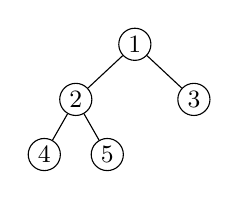
\begin{tikzpicture}[level distance=0.7cm, level 1/.style={sibling distance=1.5cm}, level 2/.style={sibling distance=0.8cm}, nodes={circle, draw, inner sep=1.5pt, font=\small}]
  \node {1}
    child { node {2}
      child { node {4} }
      child { node {5} }
    }
    child { node {3} };
\end{tikzpicture}
\end{center}
\textbf{Term Representation:} \\
\texttt{Node (Node (Node Leaf 4 Leaf) 2 (Node Leaf 5 Leaf)) 1 (Node Leaf 3 Leaf)}

\columnbreak

\textbf{Leaf-labeled Binary Trees (Alternative):}
\begin{center}
\texttt{datatype 'a tree = Leaf 'a | Node "'a tree" "'a tree"}
\end{center}

\textbf{Structure:}
Values are stored exclusively at the leaves, and internal nodes only join subtrees together.
\end{multicols}
\end{tcolorbox}

\end{document}
